\chapter{Background}

\section{Heterogeneous Architectures}
\label{sec:heterogeneous}

About why heterogeneous architectures and SHMAC are good.

% I'll write this one -KKS.

\subsection{SHMAC}
\subsection{Current Interconnect System in SHMAC}
\todo{Add reference to the SHMAC introduction paper, including pagenumber?}
%TODO Add reference to the SHMAC introduction paper, including pagenumber?
SHMAC implements a 2D mesh-based Network-on-a-Chip (NoC) interconnection network. 
Currently, the system uses dimension-ordered (XY) routing, and store-and-forward
switching with on/off flow control. The switching routine can be replaced in the
future, should the current routine be found to cause performance bottlenecks \cite{shmac-plan}.

\todo{Make sure the "goal"-part is valid}
%TODO Make sure the "goal"-part is valid
SHMAC does not implement DMA today, and data transfers are performed by the
on-tile processors. A goal of this project is to explore the option of implementing
a DMA module and testing it in a shared-bus system, before creating a prototype that
can be implemented in SHMAC.

\section{The Bitcoin Currency}
\label{sec:bitcoins}
Bitcoin is a decentralized currency using a peer-to-peer network to replace
the financial institutions that are used to process transactions in conventional
currency systems.

The network keeps a ledger of all transactions in a linked list of blocks, called the
block-chain. Each block contains a list of all transactions executed since the last
block was published. Blocks are generated periodically through a process
called ``mining'', described in \ref{sec:bitcoin-mining}. This is due to the fact that
a valid block must satisfy the requirement that the hash of the block must be below a certain value
which is determined by a variable difficulty value used to limit the number
of blocks being generated each hour \cite{bitcoin}.

As an incentive to keep generating new blocks, a reward is offered on each new block
generated. This reward is currently at 25~bitcoins (467~USD as of the 9th of November, 2014)).
This reward is why bitcoin mining is a popular activity, and a reason for why
there are many initiatives to improve the performance of bitcoin mining systems.

\subsection{Mining Bitcoins}
\label{sec:bitcoin-mining}
The process of creating a new block in the bitcoin network is called ``mining''. The basic
principle of bitcoin mining is to create a block that generates a SHA-256 hash with
a value lower than a preset target value.

Since bitcoin mining is an NP-hard problem \cite{bitcoin-np}, the search for a valid block
hash has to be done by brute-force search. The block header contains several fields
that can be varied to produce different hashes, and it is also possible to include
or exclude transactions from the block in order to produce a hash with the desired
value.

Mining performance is measured in hashes per second, denoted H/s. Hashing is the
most computing intensive part of the algorithm for mining bitcoins, which is
why accelerating hashing is a priority.

\section{Cryptographic Hashing}

A cryptographic hash function, also commonly referred to as a digital signature or
a message digest, is a function that takes input data of varying size and
produces an output value of a constant size \cite{hashing-overview}.
% That article is a pain to read, it pains me to cite it

Cryptographic hash functions are designed to be one-way, meaning it should
not be computationally feasible to find the input data given the hash value,
and collision resistant, meaning that it should not be practical to find two
different sets of input data that produces the same output hash \cite{sha-spec}.

\subsection{The SHA-256 Hashing Algorithm}

The SHA-256 algorithm is a member of the set of algorithms referred to as the SHA-2 standard.
These are described in \cite{fips180-4} and consists of algorithms for producing hashes with lengths of 224, 256, 384 and 512 bits.
The algorithms use simple operations, limited to shifts, rotates, xor, and unsigned additions,
in addition to a lookup-table of constants, which allow for high-speed implementations in both
software and hardware. The different algorithms differ in how and with what parameters the various
operations are invoked.

\subsection{SHA-256 in Detail}

SHA-256 is the algorithm used in cryptocoin mining. It operates on blocks of 512 bits
and keeps a 256-bit intermediate hash value as state.

Before the first block is processed, the initial hash value is set to a predefined
value. The entire message that is to be hashed is then padded by adding a 1 bit to
the end of the message and then appending zeroes until the length of the final block
is 448 bits. Then the length of the entire message, without padding, is added as a
64-bit big-endian integer to the end of the block.

Then, each input block is split into a 64 32-bit long expanded message block, where
each 32-bit word $W_j$ is defined according to the formula

\[ W_j = \left\{
	\begin{array}{l l}
		M_j & \quad j \in \left[0, 15\right]\\
		\sigma_1(W_{j - 2}) + W_{j - 7} + \sigma_0(W-{j - 15}) + W_{j - 15} & \quad j \in \left[16, 63\right]
	\end{array}
\right.\]

\noindent where $M_j$ is the $j$th word of the input message block and the functions
$\sigma_0$ and $\sigma_1$ are defined as

\[\sigma_0 = R^7(x) \oplus R^{18}(x) \oplus S^3(x)\]
\[\sigma_1 = R^{17}(x) \oplus R^{19}(x) \oplus S^{10}(x)\]

\noindent where the operator $R^n$ means right rotation by $n$ bits and $S^n$ means right shift by $n$
bits \footnote{Curiously, \cite{sha-spec} defines the operator $R$ as shift and $S$ as rotate.
We use the more intuitive definitions.}.

\subsubsection{The Compression Function}
The compression function is the core of the SHA-256 algorithm. It uses a look-up table
of 64 constants, $K_j$, and the following functions when calculating the new intermediate
hash values:

\[Ch(x,y,z) = (x \wedge y) \oplus (\neg x \wedge z)\]
\[Maj(x, y, z) = (x \wedge y) \oplus (x \wedge z) \oplus (y \wedge z)\]
\[\Sigma_0(x) = R^2(x) \oplus R^{13}(x) \oplus R^{22}(x)\]
\[\Sigma_1(x) = R^6(x) \oplus R^{11}(x) \oplus R^{25}(x)\]

Before starting the iterations with the compression function, the intermediate
hash values from the previous message block are assigned to the variables $a$--$h$.

At the beginning of each iteration of the compression function, two temporary
values are calculated:

\[T_1 = h + \Sigma_1(e) + Ch(e, f, g) + K_j + W_j\]
\[T_2 = \Sigma_0(a) + Maj(a, b, c)\]

The new hash values are then assigned as follows:

\[\begin{array}{l}
	h \leftarrow g \\
	g \leftarrow f \\
	f \leftarrow e \\
	e \leftarrow d + T_1\\
	d \leftarrow c \\
	c \leftarrow b \\
	b \leftarrow a \\
	a \leftarrow T_1 + T_2 \\
\end{array}\]

The compression function is run 64 times, once for each extended message block word,
$W_j$. Afterwards, the intermediate hash for the message is updated by adding the
variables $a$--$h$ to the corresponding values of the intermediate hash values from
the previous message block.

When the final input block has been processed, the final hash is composed by
concatenating the intermediate hash values \cite{sha-spec}.

\section{Direct Memory Access (DMA)}

A DMA is used to offload the transfer of blocks of data between memory locations from
the processor(s) in a system. This allows the processors to work on other tasks or enter
a sleep state while data is being transferred.

In order for a hashing accelerator to be energy efficient and have better performance,
it is important that a processor does not have to do memory transfers by itself. Therefore,
a DMA module is being designed that can be used for transferring data to or from the hashing
module, and later be extended to work as a general DMA in the SHMAC architecture.

\subsection{A Brief History of DMA}

Originally, processors polled different peripheral devices for data. This caused the processors
to enter loops where they waited for the data to be ready, which is inefficient. An alternative
to polling peripherals is using interrupts, where the processor receives an interrupt when
a device is ready for data to be read from it or written to it. This saves the processor from
having to keep polling the device for data. In both cases, however, the processor takes care
of the transfer of data to or from the device.
\todo{Insert references?}

%TODO Qualify the introduction history, of polling and interrupts. Get coverage by reference.
%\todo{Qualify the introduction history, of polling and interrupts. Get coverage by reference.}
%Originally, the processors polled the different devices for data transfer requests. Most of the time, the polls returned negative answers, and this was concidered inefficient. An alternative to polling is using interrupts, where the processor receives an interrupt from a device requesting data transfer to or from memory. This is more efficient than polling, since the processor does not have to keep polling the devices for requests. In both cases, however, the processor executes the data transfer.

% Devices do not directly ask the CPU to transfer data for them, they usually cause
% interrupts when something interesting has happened; it is then up to the CPU to
% take an action depending on what has happened. Such an action can for example be
% to transfer data to or from the peripheral. I think this should be clarified
% in the section above. -K.

Direct Memory Access was developed in 19XX\todo{Year?} to save the processor
from doing data transfer between peripheral devices. Typical use is that as soon as a
processor receives a request from a peripheral device, it activates the DMA module.
The DMA module receives a load address, a store address and a count of how much data to
transfer. While the DMA executes the data transfer, the CPU can sleep or work on other
tasks, until the DMA module signalizes that it is done.

\subsection{DMA Module Functionality}
\todo{Documentation, documentation, documentation!}
%TODO Documentation, documentation, documentation!
The minimum requirement of a DMA module is to be able to transfer data from one location to another.
However, for an efficient implementation for a given system, there are several options to consider,
such as operational modes, transfer types, integration with the rest of the system, and which
registers and interrupts to provide. The architecture of the DMA module is affected by
the options chosen, and how well they will fit in the SHMAC system.

\subsection{Operational Modes}
\todo{WARNING: Got only Wikipedia on this. Document!}
%TODO WARNING: Got only Wikipedia on this. Document!
The operational mode concerns how the DMA operates on the interconnect network, together
with other peripherals that may also need to use the network. In regular shared-bus systems,
there are three commonly used modes:

\begin{description}
    \item[Burst mode.]
    The DMA module has full ownership of the bus as long as the transfer is under execution.
    This is the fastest transfer mode for a DMA module, but it limits bus access for other
    peripherals as long as the DMA is executing the transfer.

    \item[Cycle stealing mode.]
    The DMA requests the bus as in burst mode, but relents control of the bus after transferring
    each byte of data. It will then re-request access to the bus for each transmission.
    In this way, the CPU and other peripherals can get earlier access to the bus if they need to.

    \item[Transparent mode.]
    DMA transfers data only when the CPU or other modules are not performing operations that
    require access to the bus. This is the slowest mode, but also the one that allows the best
    overall system performance.
\end{description}

In a packet-switched network, such as the one used on SHMAC, the implementations of these
principles will be different, but the principles remain the same; how high priority should
DMA transfers have, compared to other transfers in the system? Having transfers be as quick as possible,
like in the burst mode, will make DMA transfers more efficient, but will also place the
most restriction on the network for other modules and peripherals, should it occur at a
time when many peripherals or tiles are attempting to perform data transfers.

A lower priority scheme will make data transfers go faster for other modules, but at
the same time, DMA transfers will be slower. Deciding the priority of a DMA transfer,
however, will be up to the routers in the network, and is therefore outside the scope of this project.

\subsection{Transfer types}
\todo{These functions are from the manual of the PIC24F family by Microchip Inc. Add reference!}
%TODO These functions are from the manual of the PIC24F family by Microchip Inc. Add reference!
Transfer types describes how the source and destination addresses are used in the transfer.
Some commonly used options are:

\begin{description}
    \item[Fixed-to-fixed transfers.]
    Both the source and destination addresses remain the same for each data transfer.
    This mode is suitable for transfers of single data between two fixed addresses,
    or if the DMA operates with single-word transfers.
    \item[Fixed-to-block transfers.]
    The source address is fixed, while the destination address increments.
    This is useful for storing data \emph{from} the buffer of, for instance, a serial
    communication peripheral, such as the 16C750 UART.
    It could also be used to do multiple copies of data from a single address to multiple addresses.
    \item[Block-to-block transfers.]
    Both source and destination addresses increment for each transfer.
    This is the scheme where entire blocks of data is transferred during a single operation.
    \todo{Perhaps mention this as a requirement?}
    \item[Block-to-fixed transfers.]
    The source address increments, while the destination address remains the same.
    This is useful when, for instance, transferring data \emph{into} the buffer of a
    serial communications peripheral.
\end{description}

More complicated DMAs also support additional modes, such as using more complex patterns
when modifying the source and destination addresses or modifying the data in-flight.

%\subsection{System and Data Registers}
%A DMA requires minimum a buffer for storing transfering data, as well as registers for load addresses and store addresses.
%At a minimum, a DMA requires registers containing the load and store addresses.
%Counters and a register for the maximum count is also needed when transferring blocks of data.
%\todo{What is a channel?}
%DMA modules often operate with multiple channels, each handling their own data transfers.
%A possible implementation for multiple channels is to have seperate registers for load addresses, store addresses and counts for each channel.
%Another possible implementation is to have a buffer for outgoing data, where request ID, load address and store address are combined in order to recognize the incomming data from the load memory and send them to the correct store address.
%In this case, one counter may operate with one load address and generate the requests at the time.
%
% - Commented out because I don't agree on this. -K.

\subsection{DMA Integration Considerations}
\todo{Add a figure of each option}
\todo{Documentation, documentation, documentation... uhm... how do you document your separate ideas for the options?}

A DMA module may be implemented as a separate tile in SHMAC, as seen in figure \todo{Add figure} ADD FIGURE, or as an accelerator on an exisiting tile, for instance in a CPU tile, as seen in figure \todo{Add figure} ADD FIGURE.

There are different reasons for and against each option:
\begin{itemize}
    \item A full tile gives the benefit of having a full tile for the DMA implementation.
    This is useful for complex implementations that require much space.
    However, for a simple implementation, a full tile may be a waste of space.
    \item As an accelerator, a DMA module is implemented on an already existing tile.
    A tile may have parts of it powered down, therefore a DMA module may very well be implemented without any significant cost in terms of power usage.
    In fact, a DMA module may work as the only active part of a tile as well.
    A tile with a DMA module can also use the DMA to transfer data between internal modules on the tile.
    However, this also means the DMA has to share the internal shared bus network with other modules.
\end{itemize}

For a basic implementation of a DMA in SHMAC, all that is needed for the DMA module to work is that it can transfer data from one address to another.
It does not need to know where in the system it is, and what route the data must take from the load address to the store address.
Figure \ref{fig:DMASHMAC1} shows an example where the DMA is implemented on a seperate tile.

\begin{figure}[h!]
    \centering
    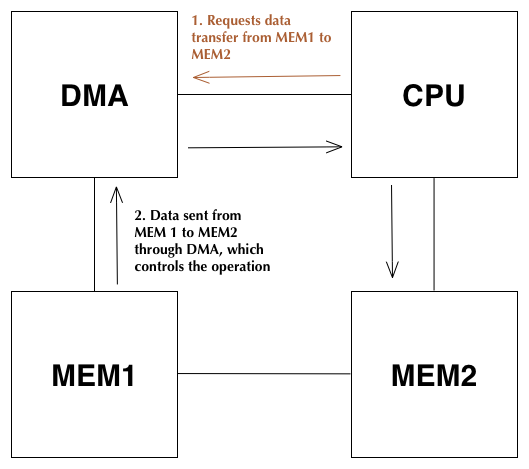
\includegraphics[width=0.7\textwidth]{Figures/DMA/DMASHMAC1}
    \caption{DMA module implemented as a tile on SHMAC, with basic transfer from MEM1 to MEM2 through itself}
    \label{fig:DMASHMAC1}
\end{figure}
\todo{Figure needs update, remove some texts and rename PU to CPU}
 
As can be seen in the figure, the DMA tile recieves a request from its neighbouring CPU tile, and performs loads and stores from the tile MEM1 to the tile MEM2.
This would also work the same way if the DMA module was implemented on the CPU tile as an accelerator instead.
While this completes the basic goal of moving data on behalf of the CPU tile, it does not know or care where in the SHMAC system it is.
If two memory tiles are close to each other, while the active DMA tile is far away (for instance on the other side of the entire SHMAC board), the data would have to travel unnecessarily far to reach the goal, and the entire operation will slow down.
Figure \ref{fig:DMASHMAC2} shows an implementation where the DMA tile tricks MEM1 to believe that MEM2 requests the data, and loads out the data while MEM2 stores the recieved data.
This could be done by sending a request signal through MEM2 to MEM1 with packet info claiming that the requestor is MEM2. 

\begin{figure}[h!]
    \centering
    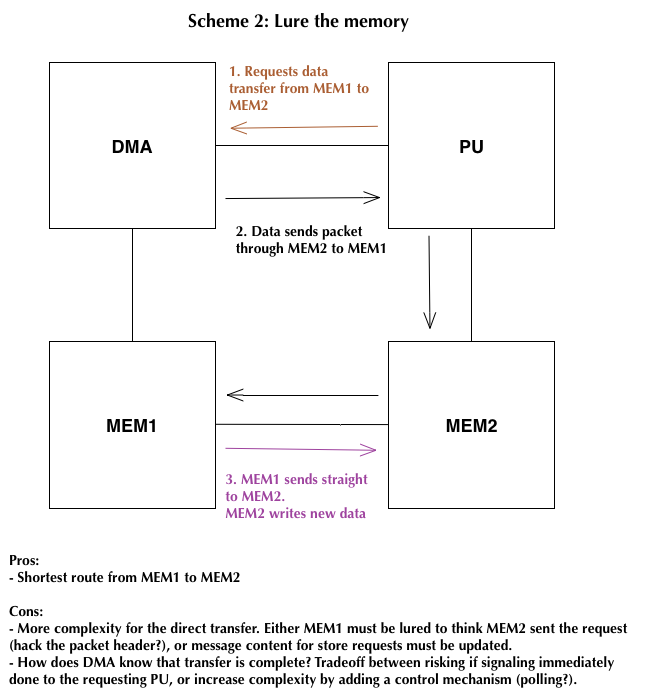
\includegraphics[width=0.7\textwidth]{Figures/DMA/DMASHMAC2}
    \caption{DMA implemented by tricking MEM1 to transfer data to MEM2}
    \label{fig:DMASHMAC2}
\end{figure}
 
This way, the distance is as short as possible, but how does the DMA tile know when the transfer is done, since it is not doing the transfer itself?
It could ignore this task and signal the CPU that the transfer is complete as soon as the tricking request has been sent out, but depending on the storing tile (a memory tile, or another accelerator tile), the CPU will risk loading old data that has not yet been overwritten, should it load from the ``wrong'' address before new data has arrived.
Alternatively, the DMA module may be implemented with polling, so that it polls the MEM2 tile to see when the data transfer is complete.
This leads to additional complexity in implementing the DMA.
 
\begin{figure}[h!]
    \centering
    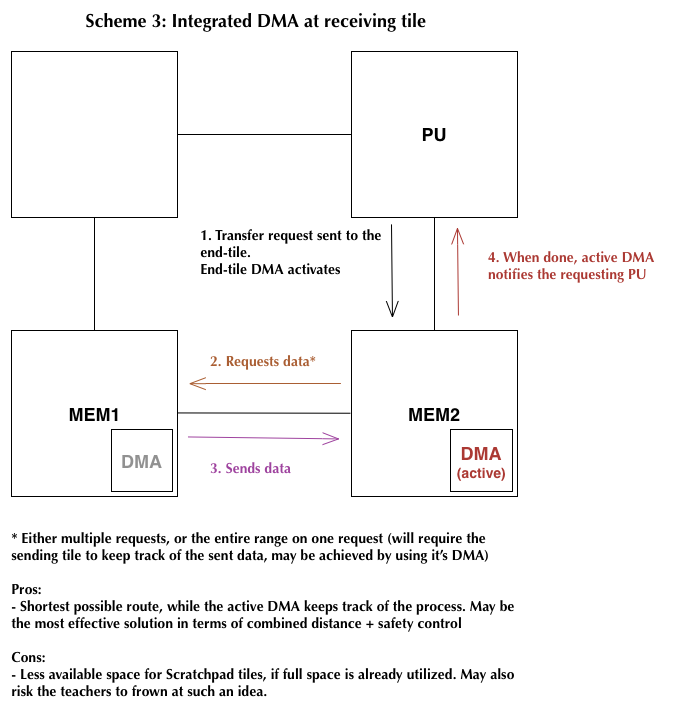
\includegraphics[width=0.7\textwidth]{Figures/DMA/DMASHMAC3}
    \caption{DMA module implemented directly on storing memory tile}
    \label{fig:DMASHMAC3}
\end{figure}
 
Figure \ref{fig:DMASHMAC3} shows an implementation where the DMA module has been implemented on the memory tiles themselves.
In this implementation, the CPU sends the DMA transfer request to the DMA on the storing tile.
As soon as the request reaches the DMA module on MEM2, it will generate load requests to MEM1.
As soon as data arrives, the DMA module will store the data in the store addresses, and signal the requesting CPU when the task is done.
The distance between MEM1 and MEM2 is kept as short as possible, and the DMA module keeps the transfer safe since it knows when the task is complete before signaling the CPU.
The main drawback is that by implementing the DMA module directly on the memory tile, there will be less space for the memory itself.

The DMA module and the entire operation will also be more complex, for a multitude of reasons;
either the DMA module itself must know where it is in the system, before either passing on the request to the correct DMA module on the correct tile, or the requesting CPU itself must know where the correct DMA module is (either by checking a look-up table, or deducing it from the destination address).
In the first case, the DMA module must be implemented with knowledge of its own position, and with the ability to pass on requests to the correct module.
This itself increases the complexity of the module.\todo{But also add favorable reasons?} 
Another question also arises: would the DMA module in MEM2 send multiple single load requests to MEM1, or should it cooperate with the DMA module on MEM1 by sending only the start address and the transfer length, and letting the module on MEM1 load and send out the data?
The latter case would be more efficient in terms of data transport, as only one request from MEM2 to MEM1 would be necessary, but at the same time, implementing a cooperation scheme between two DMA modules would further increase the complexity of the implementation.
On a memory tile, further complexity also means less memory space.
In summary, this is a compromise between memory size and efficiency.
 
%\subsection{Cache Coherency Issues}
%In SHMAC, data that is shared among more than one processing unit, are currently found only in uncachable memory areas.
%What do we do with multiple DMA writes to same uncachable area?
%TBA.
%
% - Cache coherency is not an issue when there is no cache :-) -K.

%\subsection{Issues with virtual memory}
%Currently, SHMAC does not implement virtual memory, but since it is planned to implement, it has to be addressed as well.
%It's nothing personal, Jack. It's just good business. 
%
% - Virtual memory is handled internally in the processors, the DMA operates only on physical addresses unless an IOMMU is used. -K.

%\subsection{Other options to consider}
%What is the data size? 
%Byte or bit? 
%Who can interrupt? 
%What type of interruptions may the DMA send out? 
%Multiple jobs?
%Generic DMA or specialized DMAs?
%
% - Commented out for the first draft. -K.

